\documentclass{article}
\usepackage[a4paper]{geometry}
\usepackage[spanish]{babel}
\usepackage{parskip}
\usepackage{setspace}
\usepackage{graphicx}
\usepackage{fancyhdr}
\usepackage{typearea}
\geometry{total={6in, 9in}}
\usepackage{blindtext} % no sé 
\usepackage{makeidx} % no sé 
\usepackage{lscape}
\usepackage{pdflscape}
\usepackage{fancyhdr}
\usepackage{pdfpages}
\usepackage{rotating}
\usepackage{etoolbox}
\usepackage[absolute]{textpos}


\newcommand{\tabitem}{%
  	\usebeamertemplate{itemize item}\hspace*{\labelsep}}
\usepackage[hidelinks]{hyperref}

%HEADRULE

\pagestyle{fancy}
\setlength{\headheight}{30.2pt}
\setlength{\headsep}{30pt}
% INICIO DE PÁGINAS
\begin{document}
\begin{titlepage}
	
	
	\begin{center}
		{\LARGE \textbf{UNIVERSIDAD NACIONAL DE INGENIERÍA}}\\
		\vspace{5 mm}
		{\large \textbf{Facultad de Ingeniería Industrial y de Sistemas}}\\
		\vspace{15.5 mm}
		\begin{figure}[h]
			\centering 
			
\includegraphics[width=0.45\textwidth]{images/CiberSecFIIS.png}
		\end{figure}
		\vspace{4 mm}	
		{\Large \textbf{Informes de exploración de vulnerabilidades en HTB} }\\
		\vspace{5 mm}
		
		\onehalfspacing  % Espaciamiento 1.5
		{\Large \textbf{``{\@De las máquinas: OpenAdmin, Fuse \\Magic, Remote }''} }\\
		
		\singlespacing  % Fin del espaciamiento 1.5
		
		\vspace{4 mm}	

		\vspace{20 mm}
		{\large \textbf{ELABORADO POR:} }\\
		\vspace{10 mm}
		\begin{center}
			\begin{minipage}{0.7\textwidth}
			  \begin{itemize}
				\item \Large Alfonso Suárez, Luis
				\item \Large Mottoccanche Tantaruna, Joseph
				\item \Large Chi Jon, Lau
			  \end{itemize}
			\end{minipage}
		  \end{center}

		\vspace{5 mm}	
	\end{center}

\end{titlepage}


\clearpage
\tableofcontents
\clearpage
% ----------------------------OPENADMIN-----------------------------------
\section{OpenAdmin}
\subsection{Reconocimiento}
\subsection{Escaneo de Vulnerabilidades}
\subsection{Enumeración}
\subsection{Explotación}
\subsection{Post Explotación}


\clearpage
% ----------------------------REMOTE-----------------------------------
\section{Remote}
\subsection{Reconocimiento}
Lo primero a hacer en este caso es un escaneo de nmap, para encontrar algunos puertos abiertos y servicios corriendo, en este caso se encontraron los puertos 21, 80 y 445 abiertos principalmente.

\begin{figure}[h]
	\center
	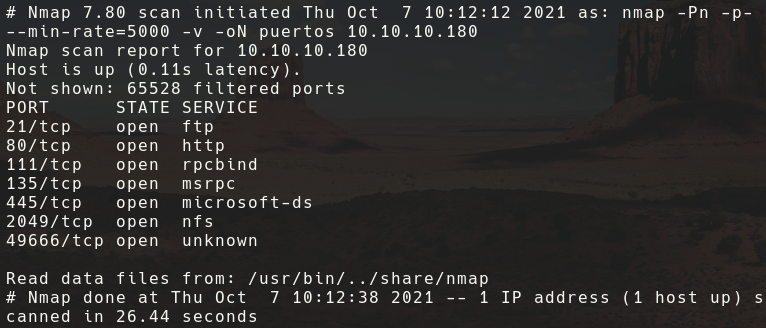
\includegraphics[width=0.8\textwidth]{images/remote/nmap_remote.png}
	\caption{nmap remote}
\end{figure}
 
\subsection{Escaneo de Vulnerabilidades}

Como primer escaneo de vulnerabilidades se intenta con el mismo nmap, con la opción "--script vuln", esto probará as vulnerabilidades más comunes en el server.

\begin{figure}[h]
	\center
	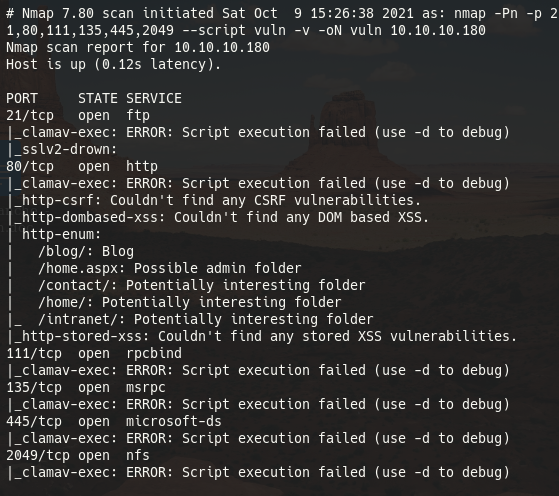
\includegraphics[width=0.7\textwidth]{images/remote/nmap_vuln.png}
	\caption{vulnerabilidades por nmap}
\end{figure}
\subsection{Enumeración}

Luego de ver los puertos, nmap no nos bota una vulnerabilidad por FTP, pero de todos modos nunca está de más probar si encontramos algo, sin embargo en esta ocasión no encontramos nada relevante.
\begin{figure}[h]
	\center 
	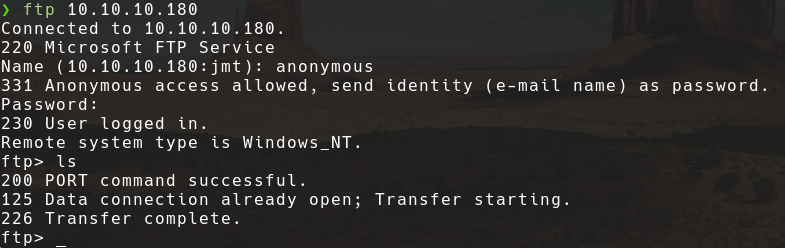
\includegraphics[width=0.8\textwidth]{images/remote/ftp.png}
	\caption{logueo anónimo por FTP}
\end{figure}

Intentamos luego con la página ubicada en el puerto 80, a ver si encontramos algo, y efectivamente encontramos una página que tiene diferentes apartados para revisar, buscamos info en los cuadros y en toda la página pero es solo texto generado de relleno, así que no hay información relevante en estas páginas para diccionarios.
\begin{figure}[h]
	\center 
	
\includegraphics[width=0.8\textwidth]{images/remote/index_pagina.png}
	\caption{logueo anónimo por FTP}
\end{figure}

\clearpage

Entre todas las páginas encontramos un apartado de login, está en el mismo servidor así que se ve bastante interesante junto a que el framework es de umbraco según el wappalizer.
\begin{figure}[h]
	\center 
	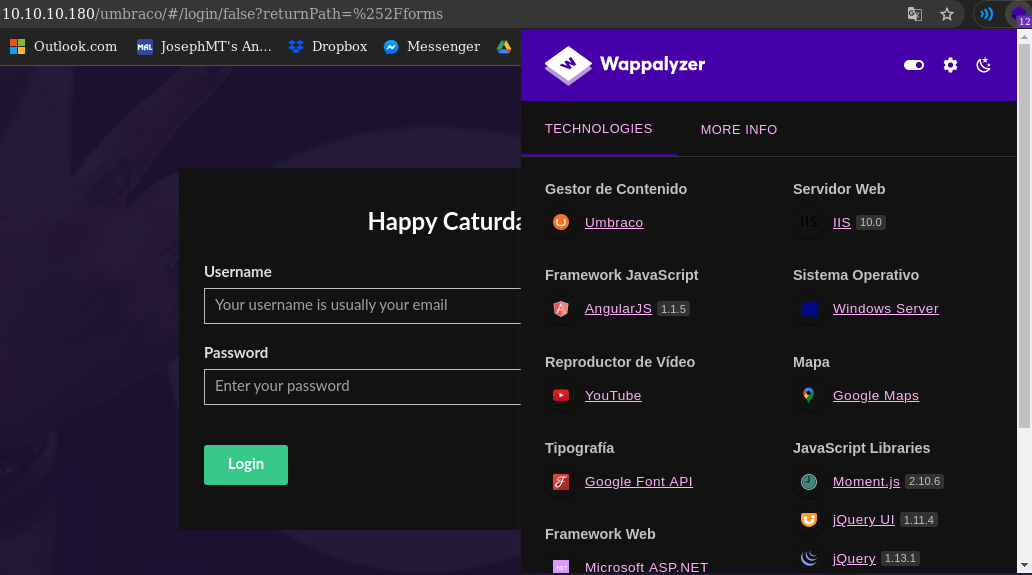
\includegraphics[width=0.8\textwidth]{images/remote/wappalizer.png}
	\caption{logueo anónimo por FTP}
\end{figure}

Intentamos un escaneo con dirb para escanear los posibles directorios ocultos, donde se encontraron muchos directorios que de forma normal hubieran sido localizados y otros que hacen referencia a redirecciones, algunos que mostraron un error de configuración pero no grave.
\begin{figure}[h]
	\center 
	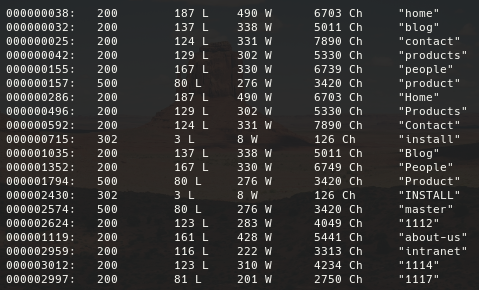
\includegraphics[width=0.8\textwidth]{images/remote/dirb.png}
	\caption{logueo anónimo por FTP}
\end{figure}


\subsection{Explotación}
\subsection{Post Explotación}

\clearpage
% ----------------------------FUSE-----------------------------------
\section{Fuse}
\subsection{Reconocimiento}
\subsection{Escaneo de Vulnerabilidades}
\subsection{Enumeración}
\subsection{Explotación}
\subsection{Post Explotación}

\end{document}
